% !TEX root = ../paper.tex

\section{Materials and Methods}				% 2-5 pages

%%%	Materials & Methods: the "how" section (2-5 pages)
%%%		Describe how you performed your work, giving sufficient detail so that someone trained in the field is able to understand what you did and can replicate it.
%%%		Include the methods you used, written in a format commonly used in publications in your field of study.
%%%		Do not merely restate a protocol or copy blocks of text; instead, use your own words to describe what you did, referencing key papers where appropriate.
%%%		Explain your personal role in the work and the roles played by others in supporting this work.
%%%		Include, for example, acknowledgments to others in the laboratory for running key instrumentation or other protocols.
%%%		You may refer to others who assisted you by title but do not include any specific names in the body of your Research Report.
%%%		Mention common procedures but there is no need to describe them in detail; provide references to where the method is published.
%%%		All modifications of existing methods should be described.

\subsection{High Level Process}
\vspace{1ex}
\begin{onehalfspacing}
	\begin{enumerate}
		\item A master quadrotor drone captures high altitude imagery of an area by automatically navigating between generated GPS waypoints.
		\item Servers identify SIFT keypoints and stitch images together into map overlays.
		\item Slave quadrotor drones are deployed to keypoint clusters and capture high resolution panoramas.
		\item Indoor 3D maps are generated with drone mounted RGBD cameras.
	\end{enumerate}
\end{onehalfspacing}

\subsection{AR.Drone}

We modified the $\$300$ Parrot AR.Drone 2.0 recreational quadrotor to serve as a base payload carrying platform. The lightweight drone is very inexpensive, although we had to strip much of the protective casing to increase additional cargo capacity. The UAV has a built in frontal camera, with a resolution of $720$p ($1280$×$720$) and a $240$p QVGA high frame rate bottom stabilization camera. The AR.Drone includes a logic board that coordinates the four rotors and stabilizes the craft with sensory input.

Summary of UAV specifications\cite{ardrone2:specs}:
\begin{onehalfspacing}
	\begin{itemize}
		\item Barometer and ultrasonic sensor for altitude measurement
		\item Accelerometer and gyroscope
		\item $1280$×$720$ pixel wide angle front camera
		\item $320$×$240$ pixel QVGA high frame rate bottom camera for measuring ground speed
	\end{itemize}
\end{onehalfspacing}


\textbf{By using off the shelf hardware and modifying it for the project requirements, the price per drone can be kept low due to price savings from large scale mass production}.

\subsubsection{UAV Control}

\begin{onehalfspacing}
	\begin{enumerate}
		\item An operator draws a flight path in Google Earth and way-points are generated. (\autoref{fig:FlightPlan})
		\item The drone is launched and stabilized.
		\item Photos and telemetry collected and transmitted to server.
		\item Flight is adjusted when the drone exits a 3 meter wide corridor between way-points.
		\item The flight plan is sent to the central server to be added as an imaging to the task queue for the drone fleet to deploy a charged UAV.
	\end{enumerate}
\end{onehalfspacing}

\begin{figure}[h!]
	\begin{minipage}{.4\textwidth}
		\caption{Google Earth flight plan}
		\label{fig:FlightPlan}
		\centering 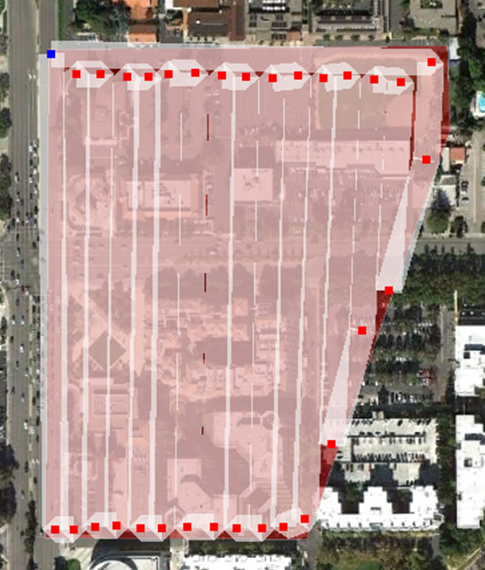
\includegraphics[width=0.9\linewidth]{illustrations/flight_path}
	\end{minipage}%
	\begin{minipage}{.6\textwidth}
		\caption{UAV control flow}
		\label{fig:DroneControl}
		\centering 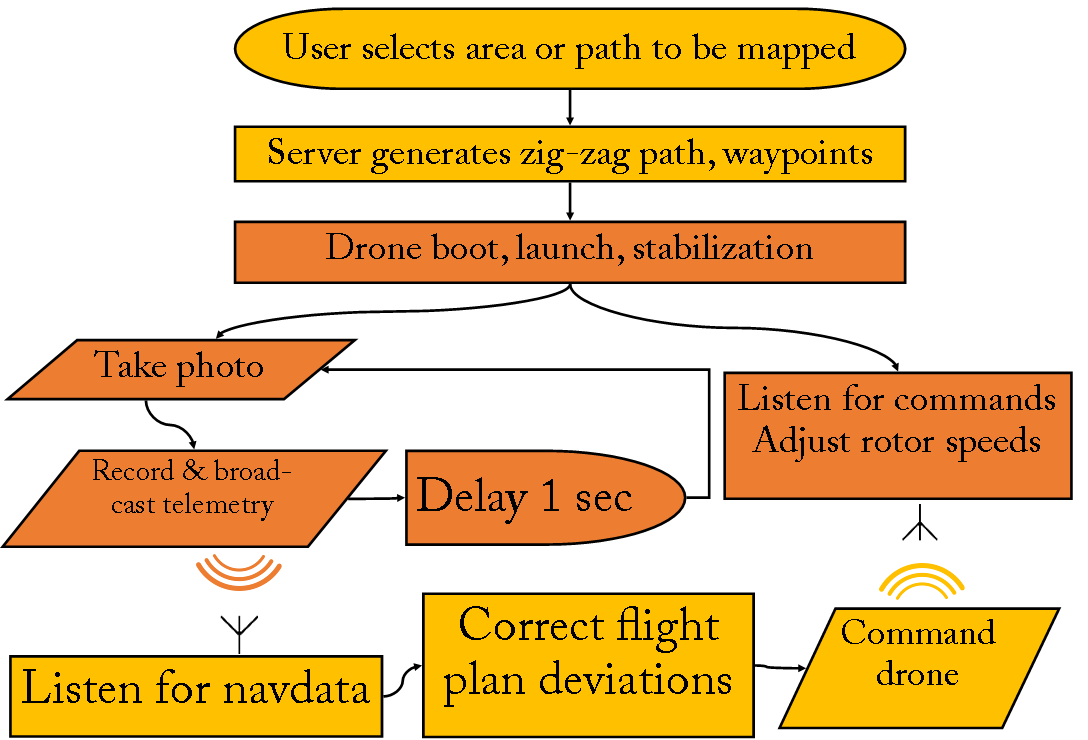
\includegraphics[width=0.9\linewidth]{illustrations/drone_chart}
	\end{minipage}
\end{figure}

\subsection{Central Server}

\begin{figure}[h!]
		\caption{Server Cluster Architecture}
		\label{fig:ServerArch}
		\centering 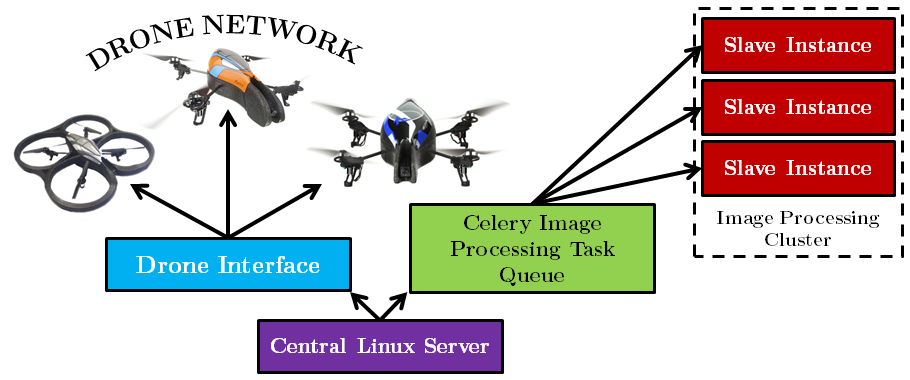
\includegraphics[width=0.9\linewidth]{illustrations/serverarch_lmroman}
\end{figure}

\noindent
A central Linux server acts as a central hub to which every drone connects to. This server handles drone management and acts as a load balancer to the rest of the cluster. As images are collected, it adds tasks to a Celery task queue. Server instances are dynamically created to complete the tasks in the Celery task queue. Such tasks include (but are not limited to) stitching, SIFT keypointing, locating faces and skin tone isolation.

Tasks are completed as a priority queue, allowing image processing jobs that are important (e.g. low resolution keypointing) to be completed first. This distributed system allows the system to become near-infinitely scalable by adding more workers. This process can be automated with a cloud service provider like the Amazon AWS Elastic Compute Cloud where new servers are dynamically provisioned as needed.



\subsection{Phone Telemetry and Ground Imaging}
\textbf{Our final prototype used an inexpensive Android smartphone with a GPS sensor and a 3G data connection to record high resolution imagery and transmit telemetry.} For development, we used the Nexus S, although cheaper and more lightweight devices could easily be substituted. With our \textit{Drone Logger} Android application, an image from the back camera (facing downward when mounted on the UAV) are recorded every second to the phone's internal storage. Depending on the specific device used, different sets of telemetry are available; we captured and transmitted the \textbf{bearing, speed, latitude and longitude}.

% is this the best place to put this? ->
Telemetry is sent to a local or remote server with a public IP address as an HTTP POST request. If telecommunications infrastructure is damaged and a data connection is unavailable on the phone, a portable server and the mounted phone would connect to an adhoc WIFI network.
The AR.Drone creates an In the development of our prototypes, the smartphone, UAV creates a local network with an approximate range of 165 meters.

\subsection{Prototypes}

\subsubsection{V1 $-$ Drone bottom stabilization camera}
Our initial prototype relied on the bottom facing stabilization camera bundled with the AR Drone. Using it for map creation would have minimized the overall costs, but the camera is of too low resolution ($240$p) for workable imagery.

\subsubsection{V2 $-$ Drone Mounted Arduino and Sensors (\autoref{fig:ArduinoDrone})}
To add cameras and additional sensors to the UAV, we mounted an Adruino microcontroller. This gave us the freedom to add additional sensors. However, the asymmetric weight distribution made the drone:
\begin{itemize}
	\item Difficult to isolate issues and to use serial communication
	\item Unstable when mounted
\end{itemize}

\subsubsection{V3 $-$ Android Smartphone and PC Server}
We overcame cost, data transmission and aerodynamic issues in previous prototypes by mounting an Android smartphone on the bottom of the UAV. The phone has several benefit to a custom Adruino based system:
\begin{enumerate}
	\item Even low-end phones contain many built in sensors, including a GPS and 3G antenna.
	\item The back camera is far superior to the built in stabilization camera of the AR.Drone
	\item Electronics are self-contained, reducing drag on the UAV.
	\item We are able to use the Android APIs to interface with sensors.
	\item The data connection allows the phone to relay telemetry data and receive instructions from a remote server.
\end{enumerate}

However, the heavy phone ($129$ grams) decreased the battery life of the UAV and the maximum altitude. To increase the cargo capacity of the AR.Drone, we removed the drone hull and phone casing. We experimented with increasing lift with helium balloons, as a a $30$ cm balloon can lift $14$ grams.
